%! Author = lazza
%! Date = 10/04/2022

\section{Introduction}\label{sec:introduction}

\subsection{Flynn Taxonomy}\label{subsec:taxonomy}
\begin{itemize}
    \item[] \textbf{Single instruction:} only one instruction stream is being acted on by the CPU during any one clock
    cycle.
    \item[] \textbf{Single data:} only one data stream is being used as input during any one clock cycle.
    \item[] \textbf{Multiples instruction:} every processor may be executing a different instruction stream.
    \item[] \textbf{Multiple Data:} every processor may be working with a different data stream.
\end{itemize}


\begin{itemize}
    \item SISD - Single Instruction Single Data – Uniprocessor systems
    \item MISD - Multiple Instruction Single Data\\
    No practical configuration and no commercial systems.
    \item SIMD - Single Instruction Multiple Data\\
    Simple programming model, low overhead, flexibility, custom integrated circuits.
    \item MIMD - Multiple Instruction Multiple Data\\
    Scalable, fault tolerant, off-the-shelf micros.
\end{itemize}

\subsection{Parallelism}\label{subsec:parallelism}
The SISD architecture is the oldest and provides deterministic execution.
To account for events happening simultaneously we have to introduce parallelism.

The SIMD, parallel architecture, with multiple data each processing unit can operate on a different data element.
Best suited for specialized problems characterized by a high degree of regularity, such as graphics/image processing.

The MIMD, nowadays, the most common type of parallel computer, execution can be synchronous or asynchronous,
deterministic or non-deterministic.\\

Type of parallelism:
\begin{itemize}
    \item DLP, data-level parallelism (SIMD)
    \item ILP, instruction-level parallelism (SIMD + pipeline)
    \item TLP, thread-level parallelism (MIMD)
    \item RLP, request-level parallelism (MIMD)
\end{itemize}

\subsubsection{Instruction-Level Parallelism}
Pipelining

\subsubsection{Thread-Level Parallelism}
Explicit parallelism implies structuring the applications into concurrent and communicating tasks.
Operating systems offer support for different types of tasks.
The most important and frequent are:
\begin{itemize}
    \item processes
    \item threads
\end{itemize}

The operating systems implement multitasking differently based on the characteristics of the processor.
Multithreading categories:
\begin{itemize}
    \item single core
        \subitem superscalar\\
    A superscalar processor is a CPU that implements a form of parallelism called instruction-level parallelism within a
    single processor.
    In contrast to a scalar processor, which can execute at most one single instruction per clock
    cycle, a superscalar processor can execute more than one instruction during a clock cycle by simultaneously
    dispatching multiple instructions to different execution units on the processor.
    It therefore allows more throughput (the number of instructions that can be executed in a unit of time) than would
    otherwise be possible at a given clock rate.
    Each execution unit is not a separate processor (or a core if the processor is a multi-core processor), but an
    execution resource within a single CPU such as an arithmetic logic unit.
    In Flynn's taxonomy, a single-core superscalar processor is classified as an SISD processor, though a single-core
    superscalar processor that supports short vector operations could be classified as SIMD (single instruction stream,
    multiple data streams).
    A multi-core superscalar processor is classified as an MIMD processor (multiple instruction streams, multiple data streams).
    While a superscalar CPU is typically also pipelined, superscalar and pipelining execution are considered different performance
    enhancement techniques.
    The former executes multiple instructions in parallel by using multiple execution units, whereas the latter executes
    multiple instructions in the same execution unit in parallel by dividing the execution (instruction) unit into
    different phases.
        \subitem multiprocessing\\

    \item single core with multithreading support
        \subitem Fine grained multithreading:
            \subsubitem item Switches from one thread to the other at each instruction
            \subsubitem the execution of more threads is interleaved (often the switching is performed taking turns,
            skipping one thread if there is a stall)
            \subsubitem The CPU must be able to change thread at every clock cycle.
            It is necessary to duplicate the hardware resources.
        \textrightarrow Advantage is it can hide both short and long stalls, since instructions from other threads executed
    when one thread stalls
        \textrightarrow Disadvantage is it slows down execution of individual threads, since a thread ready to execute
    without stalls will be delayed by instructions from other threads
        \subitem Coarse grained multithreading
            \subsubitem switching from one thread to another occurs only when there are long stalls – e.g., for a miss on
    the second level cache.
            \subsubitem Two threads share many system resources (e.g., architectural registers), the switching from one thread
    to the next requires different clock cycles to save the context.
        \textrightarrow Advantage: in normal conditions the single thread is not slowed down\\
    – Relieves need to have very fast thread-switching\\
    – Doesn’t slow down thread, since instructions from other threads issued only when the thread encounters a costly
    stall\\
        \textrightarrow Disadvantage: for short stalls it does not reduce the throughput loss – the CPU starts the
    execution of instructions that belonged to a single thread, when there is one stall it is necessary to empty the
    pipeline before starting the new thread

        TLP (e.g., superscalar) and ILP (pipelining) exploit two different kinds of parallel structure in a program
        • Could a processor oriented at ILP to exploit TLP?
        – functional units are often idle in data path designed for ILP because of either stalls or dependences in the code
        • Could the TLP be used as a source of independent instructions that might keep the processor busy during stalls?
        • Could TLP be used to employ the functional units that would otherwise lie idle when insufficient ILP exists?
        \subitem Simultaneous Multithreading (SMT)
        • The system can be dynamically adapted to the environment, allowing (if possible) the execution of instructions
        from each thread, and allowing that the instructions of a single thread used all functional units if the other
        thread incurs in a long latency event.
        • More threads use the issues possibilities of the CPU at each cycle;
        ideally, the exploitation of the issues availabilities is limited only by the unbalance between resources
        requests and availabilities.

    \item multicore
\end{itemize}

\begin{figure}
    \centering
    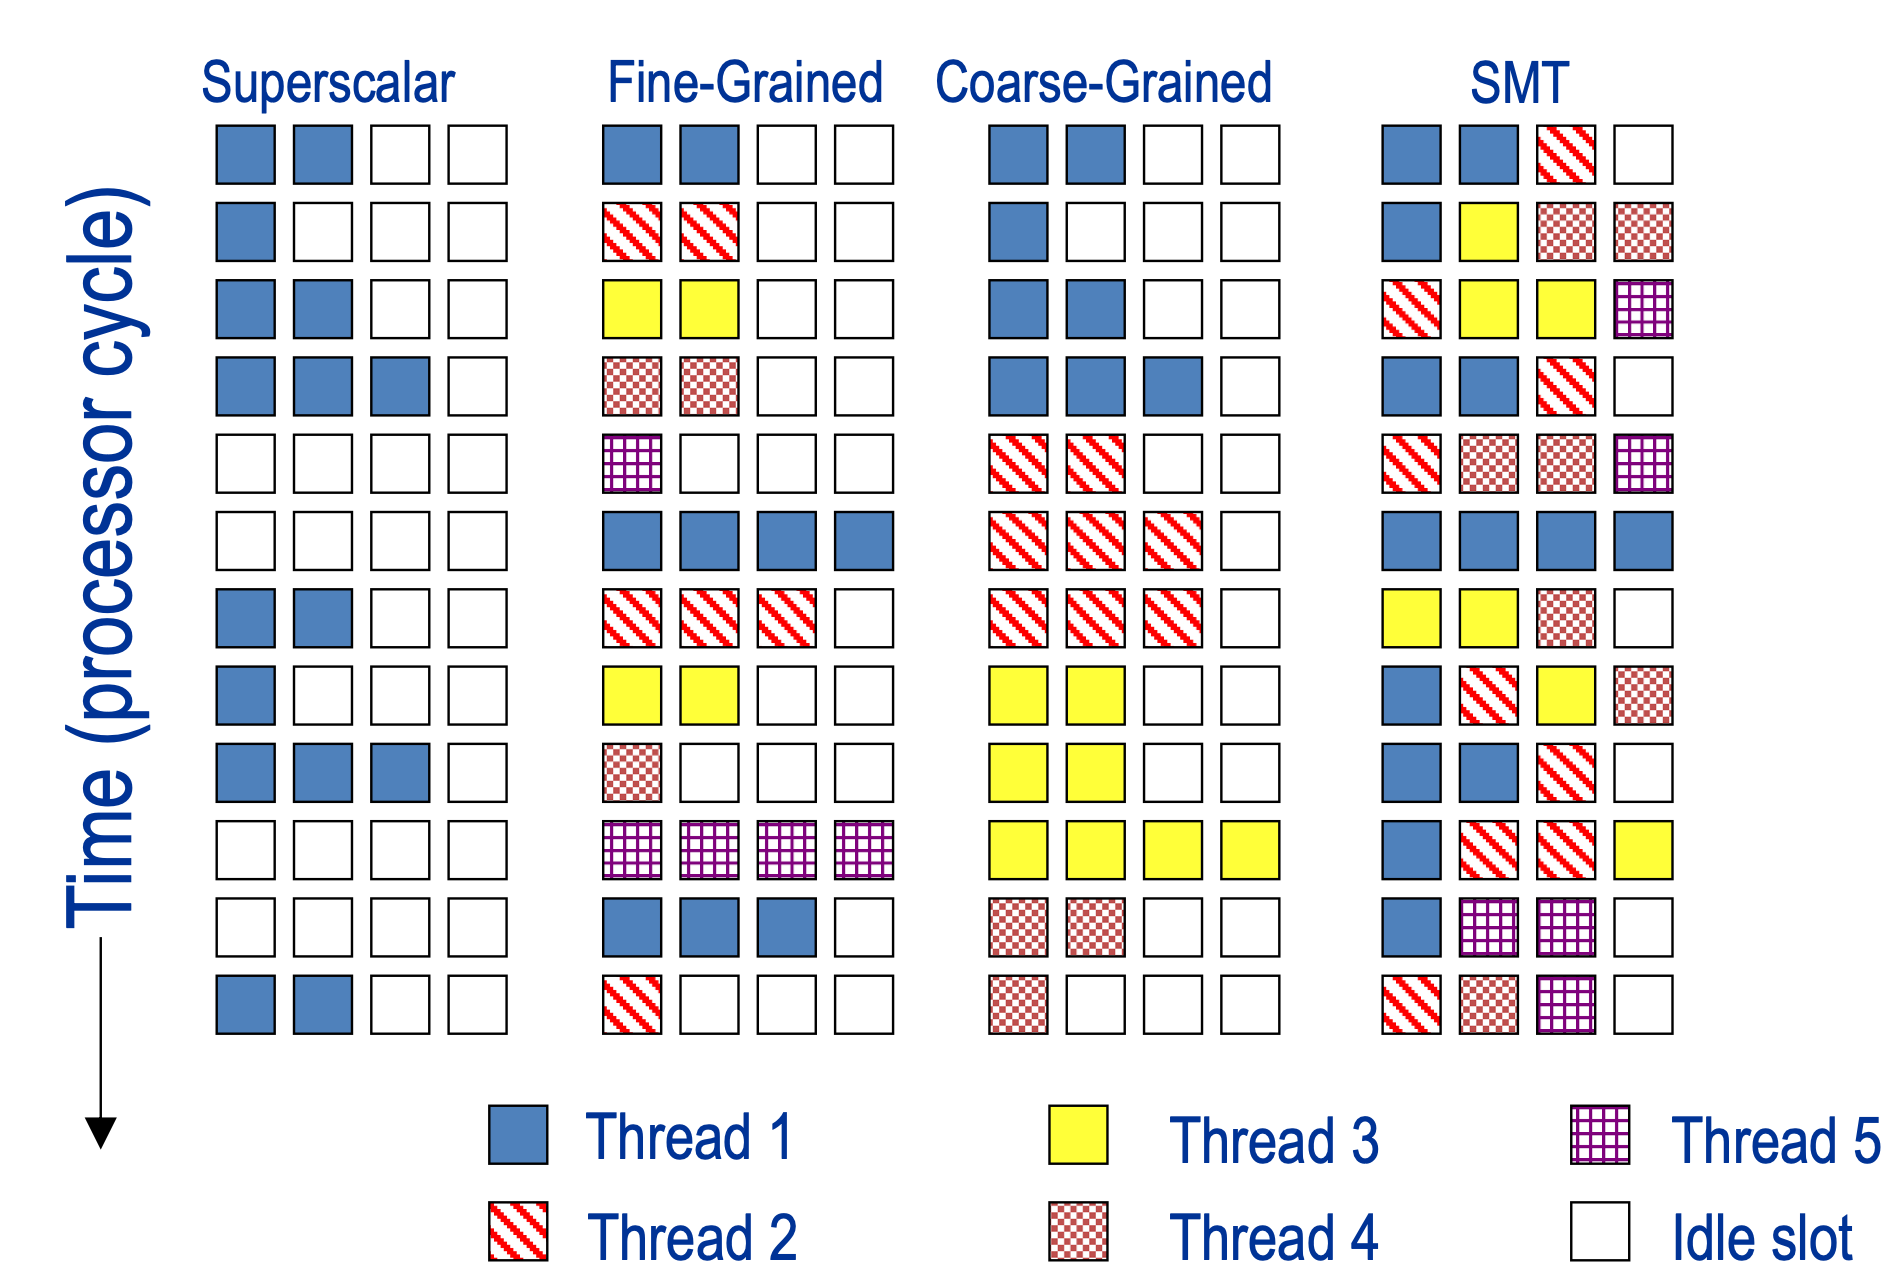
\includegraphics[scale=0.25]{images/multithreaded-categories}
    \caption{Multithreaded categories}
    \label{fig:multithreaded-categories}
\end{figure}



